% Source: Lecture16.pdf, pages 1-6 (page 1 is a title page; page 7 is blank).
% Title on the source: "Lecture 16 - Renormalization group and critical phenomena, continued".
\lecture{16}

In the previous lecture, we noted that because the linearized matrix $M$ describing the RG at the critical
point is not, in general, symmetric, the eigenvectors $\hat{\mathbf e}_1$ and $\hat{\mathbf e}_2$ are not
orthogonal. Recall the setup: in the illustrative example we had 2 couplings, $K_1$ and $K_2$; under the
(real-space) RG transformation, in the vicinity of the critical point $(K_1^*,K_2^*)$ (RGFP),
\begin{equation}
  K_1' = R_1(\{K_1,K_2\}),\qquad K_2' = R_2(\{K_1,K_2\}),
\end{equation}
\begin{equation}
  K_1' = R_1(K_1^*+\delta K_1,K_2^*+\delta K_2) = K_1^* + \left(\pder{R_1}{K_1}\right)_*\delta K_1 + \left(\pder{R_1}{K_2}\right)_*\delta K_2,
\end{equation}
similarly with $K_2$ (where $*$ means evaluated at the critical point), so with
$\delta K_i'\equiv K_i'-K_i^*$, $i = 1,2$,
\begin{equation}
  \begin{pmatrix}\delta K_1'\\ \delta K_2'\end{pmatrix}
  = \underbrace{\begin{pmatrix}\pder{R_1}{K_1} & \pder{R_1}{K_2}\\[4pt] \pder{R_2}{K_1} & \pder{R_2}{K_2}\end{pmatrix}_*}_{M}
    \begin{pmatrix}\delta K_1\\ \delta K_2\end{pmatrix}.
\end{equation}
Diagonalizing $M$: $M\hat{\mathbf e}_i = \lambda_i\hat{\mathbf e}_i$, $i = 1,2$, $\lambda_i = b^{y_i}$;
$\lambda_i>1\Leftrightarrow y_i>0$: relevant parameter, RG flow away from the RGFP;
$\lambda_i<1\Leftrightarrow y_i<0$: irrelevant parameter, RG flow into the RGFP
($\lambda_i = 1\Leftrightarrow y_i = 0$, marginal).

Since $M^T\ne M$ in general, $\hat{\mathbf e}_1$ and $\hat{\mathbf e}_2$ are not orthogonal. Let us show the
proof of this. Let $v$, $w$ be vectors in a real vector space $V$ and let $A:V\to V$ be a linear
transformation of $V\to V$. Then if $A^T = A$:

\paragraph{Theorem.} For $A:V\to V$ a real symmetric matrix, $A^T = A$, the diagonalization of $A$ has the
property that if $e_i$ and $e_j$ are two eigenvectors of $A$ with different eigenvalues, then
$\langle e_i,e_j\rangle = 0$ (where the inner product of $v$ and $w\in V$ is denoted
$\langle v,w\rangle$). The diagonalization is done with an orthogonal transformation $R$:
$R^T = R^{-1}$:
\begin{equation}
  RAR^T = RAR^{-1} = A_{\text{diag}} = \begin{pmatrix}\lambda_1 & & 0\\ & \ddots & \\ 0 & & \lambda_N\end{pmatrix}.
\end{equation}

\paragraph{Proof.} Calculate $\langle e_j,Ae_i\rangle = \lambda_i\langle e_j,e_i\rangle$. Recall that
$\langle v,Aw\rangle = \langle A^Tv,w\rangle$. Here,
$\langle e_j,Ae_i\rangle = \langle A^Te_j,e_i\rangle = \langle Ae_j,e_i\rangle = \lambda_j\langle e_j,e_i\rangle$,
so $\lambda_i\langle e_j,e_i\rangle = \lambda_j\langle e_j,e_i\rangle$, but $\lambda_i\ne\lambda_j$, so the only
solution is $\langle e_j,e_i\rangle = 0$, i.e.\ $e_i\perp e_j$.

\subsection{RG for the 1D Ising model in Boltzmann variables}

In the previous lecture, we carried out an RG analysis of the 1D zero-field Ising model. With no loss of
generality, we took $J>0$ (FM $J$), so $K\ge 0$. We derived the RG
\begin{equation}
  v' = v^2,\quad\text{i.e.}\quad \tanh K' = (\tanh K)^2,\qquad
  K' = \operatorname{arctanh}\left((\tanh K)^2\right) = \tfrac12\ln(\cosh(2K)),
\end{equation}
using $\operatorname{arctanh}x = \frac12\ln\left(\frac{1+x}{1-x}\right)$, so $K'<K$ if $0<T<\infty$.

\begin{diagram}
\begin{tikzpicture}[scale=0.9,>=Stealth]
  \draw (0,0) -- (5,0);
  \foreach \x in {0.7,1.7,2.7,3.7} \draw[->] (\x,0) -- (\x+0.4,0);
  \fill[red] (0,0) circle (0.08); \fill[blue] (5,0) circle (0.08);
  \node[above,font=\small] at (0,0.1) {$T$: $0$}; \node[above,font=\small] at (5,0.1) {$\infty$};
  \node[below,font=\small] at (0,-0.1) {$K$: $\infty$}; \node[below,font=\small] at (5,-0.1) {$0$};
  \begin{scope}[xshift=7cm]
  \draw (0,0) -- (5,0);
  \foreach \x in {0.7,1.7,2.7,3.7} \draw[->] (\x,0) -- (\x+0.4,0);
  \fill[red] (0,0) circle (0.08); \fill[blue] (5,0) circle (0.08);
  \node[above,font=\small] at (0,0.1) {$U$: $0$}; \node[above,font=\small] at (5,0.1) {$1$};
  \node[below,font=\small,align=center] at (0,-0.1) {$K = \infty$\\ $T = 0$};
  \node[below,font=\small,align=center] at (5,-0.1) {$K = 0$\\ $T = \infty$};
  \end{scope}
\end{tikzpicture}
\diagramcaption{The zero-field RG flow in $T$ and $K$ (left) and in $U$ (right).}
\end{diagram}

Recall the Boltzmann variable $z\equiv e^{-2K}$. Define
\begin{equation}
  U\equiv z^2 = e^{-4K}
\end{equation}
(lower-case in the handwritten notes; don't confuse with the internal energy $U$): $U = 1$ if $K = 0$, i.e.\
$T = \infty$; $U = 0$ if $K = \infty$, i.e.\ $T = 0$. Recasting the RG transformation in terms of $U$, we
have
\begin{equation}
  U' = \frac{4U}{(1+U)^2};
\end{equation}
proof:
\begin{equation}
  \frac{4U}{(1+U)^2} = \frac{4}{[U^{-1/2}(1+U)]^2} = \frac{4}{[U^{-1/2}+U^{1/2}]^2}
  = \frac{4}{(e^{2K}+e^{-2K})^2} = \frac{1}{[\cosh(2K)]^2},
\end{equation}
so $U' = e^{-4K'} = \frac{1}{[\cosh(2K)]^2}$, $-4K' = -2\ln[\cosh(2K)]\Rightarrow K' = \frac12\ln[\cosh(2K)]$.
It is convenient to use the Boltzmann variable because the RG transformation is an algebraic (rational)
function for $U\to U'$ but a transcendental function for $K\to K'$.

\subsection{The 1D Ising model in a magnetic field}

Now generalize the RG analysis to the full 1D Ising model with nonzero external magnetic field $H$. Define
another Boltzmann variable
\begin{equation}
  \mu = e^{-2h},\qquad h = \beta H .
\end{equation}
Take $H>0$ without loss of generality. Carry out the RG transformation with blocking parameter $b = 2$,
summing over the spins $\sigma_i$ on odd-$i$ sites of the original lattice to get the blocked lattice and the
associated $\Ham'$.

\begin{diagram}
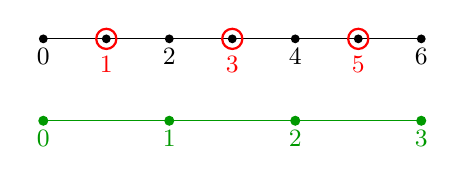
\begin{tikzpicture}[scale=0.8]
  \draw (0,0) -- (6,0);
  \foreach \x in {0,...,6} \fill (\x,0) circle (0.07);
  \foreach \x in {0,2,4,6} \node[below,font=\small] at (\x,0) {$\x$};
  \foreach \x in {1,3,5} {\draw[red,thick] (\x,0) circle (0.16); \node[below,red,font=\small] at (\x,-0.12) {$\x$};}
  \begin{scope}[yshift=-1.3cm]
  \draw[green!60!black] (0,0) -- (6,0);
  \foreach \x/\l in {0/0,2/1,4/2,6/3} {\fill[green!60!black] (\x,0) circle (0.08); \node[below,green!60!black,font=\small] at (\x,0) {$\l$};}
  \end{scope}
\end{tikzpicture}
\diagramcaption{Decimation with $b = 2$: the spins on the circled odd sites are summed over, leaving the
blocked lattice (green).}
\end{diagram}

The partition function, expressed in terms of $\sigma$'s on even and odd sites of the original lattice, is
\begin{align}
  Z &= \sum_{\{\sigma_i\}}e^{-\beta\Ham}
     = \sum_{\{\sigma_i\}}\prod_{i,j}\exp\left[K\sum_{e_{ij}}\sigma_i\sigma_j + h\sum_i\sigma_i\right]\nonumber\\
    &= \sum_{\{\sigma_{\text{even}}\}}\sum_{\{\sigma_{\text{odd}}\}}\prod_{i,j}
       \exp\left[K\sigma_i(\sigma_{i-1}+\sigma_{i+1}) + h\sigma_i + \tfrac h2(\sigma_{i-1}+\sigma_{i+1})\right],
\end{align}
where $i$ is odd and $i\pm1$ are even sites. Now perform the sums over $\sigma_i = \pm1$ on all odd sites:
\begin{align}
  Z &= \sum_{\{\sigma_{\text{even}}\}}\prod_{\text{sites}}\left\{e^{K(\sigma_{i-1}+\sigma_{i+1})+h}
       + e^{-K(\sigma_{i-1}+\sigma_{i+1})-h}\right\}e^{\frac h2(\sigma_{i-1}+\sigma_{i+1})}\nonumber\\
    &= \sum_{\{\sigma_j\}}\prod_j\exp\left[K'\sigma_j\sigma_{j+1} + h'\sigma_j + C'\right],
\end{align}
where now the $j$'s are sites on the blocked lattice. This yields the RG transformation
$(K,h,C)\to(K',h',C')$ (take $C = 0$), and $C'$ is a constant that does not have any effect on the physics,
since it divides out in all thermal averages: for any operator $\mathcal O$,
\begin{equation}
  \ev{\mathcal O} = \frac{\sum_\sigma\mathcal Oe^{-\beta\Ham}}{\sum_\sigma e^{-\beta\Ham}}
  = \frac{\sum_\sigma\mathcal Oe^{-\beta\Ham+C'}}{\sum_\sigma e^{-\beta\Ham+C'}}.
\end{equation}
Thus
\begin{equation}
  \left\{e^{K(\sigma_{i-1}+\sigma_{i+1})+h} + e^{-K(\sigma_{i-1}+\sigma_{i+1})-h}\right\}e^{\frac h2(\sigma_{i-1}+\sigma_{i+1})}
  = e^{K'\sigma_j\sigma_{j+1} + \frac{h'}{2}(\sigma_j+\sigma_{j+1}) + C'} .
\end{equation}
Evaluate this for all the possible cases for $\sigma_j$, $\sigma_{j+1}$:
\begin{align}
  \sigma_{i-1} = \sigma_{i+1} = +1,\ \text{i.e.}\ \sigma_j = \sigma_{j+1} = +1:&\quad
    e^{2K+2h} + e^{-2K} = e^{K'+h'+C'} && \text{(eq.\ 1)}\\
  \sigma_{i-1} = \sigma_{i+1} = -1,\ \text{i.e.}\ \sigma_j = \sigma_{j+1} = -1:&\quad
    e^{-2K} + e^{2K-2h} = e^{K'-h'+C'} && \text{(eq.\ 2)}\\
  \sigma_{i-1} = -\sigma_{i+1} = \pm1,\ \text{i.e.}\ \sigma_j = -\sigma_{j+1} = \pm1:&\quad
    e^h + e^{-h} = e^{-K'+C'} && \text{(eq.\ 3)}
\end{align}
(eq.~1)/(eq.~2):
\begin{equation}
  e^{2h'} = \frac{e^{2K+2h}+e^{-2K}}{e^{2K-2h}+e^{-2K}}
  = \frac{e^h(e^{2K+h}+e^{-2K-h})}{e^{-h}(e^{2K-h}+e^{-2K+h})}
  = e^{2h}\frac{\cosh(2K+h)}{\cosh(2K-h)},
\end{equation}
so
\begin{equation}
  h' = h + \frac12\ln\left[\frac{\cosh(2K+h)}{\cosh(2K-h)}\right]>h:
\end{equation}
the RG flow is to larger $h$, i.e.\ smaller $\mu = e^{-2h}$.

(eq.~1)(eq.~2)/(eq.~3)$^2$:
\begin{align}
  \frac{e^{2K'+2C'}}{e^{-2K'+2C'}} = e^{4K'}
  &= \frac{e^h(e^{2K+h}+e^{-2K-h})e^{-h}(e^{2K-h}+e^{-2K+h})}{(e^h+e^{-h})^2}\nonumber\\
  &= \frac{\cosh(2K+h)\cosh(2K-h)}{\cosh^2h},
\end{align}
so
\begin{equation}
  K' = \frac14\ln\left[\frac{\cosh(2K+h)\cosh(2K-h)}{\cosh^2h}\right].
\end{equation}
So we have calculated the RG transformation $(K,h)\to(K',h')$ (independent of the constants $C$, $C'$,
since these do not affect the physics). Also, (eq.~1)(eq.~2)(eq.~3)$^2$:
\begin{align}
  e^{4C'} &= e^h(e^{2K+h}+e^{-2K-h})e^{-h}(e^{2K-h}+e^{-2K+h})(e^h+e^{-h})^2\nonumber\\
          &= 2^4\cosh(2K+h)\cosh(2K-h)\cosh^2h .
\end{align}

It is again convenient to reexpress these RG transformation equations in terms of the Boltzmann variables
$U$ and $\mu$; the resultant equations are algebraic rather than transcendental:
\begin{align}
  e^{-4K'} = U' &= \frac{(e^h+e^{-h})^2}{(e^{2K+h}+e^{-2K-h})(e^{2K-h}+e^{-2K+h})}\nonumber\\
   &= \frac{e^{2h}(1+e^{-2h})^2}{e^{2h}\cdot e^{4K}(1+e^{-4K-2h})(e^{-2h}+e^{-4K})},\nonumber\\
  U' &= \frac{U(1+\mu)^2}{(1+U\mu)(\mu+U)},\\
  \mu' = e^{-2h'} &= \frac{e^{2K-2h}+e^{-2K}}{e^{2K+2h}+e^{-2K}}
   = \frac{e^{2K}(e^{-2h}+e^{-4K})}{e^{2K+2h}(1+e^{-4K}e^{-2h})}\nonumber\\
   &= \mu\left(\frac{\mu+U}{1+U\mu}\right).
\end{align}
So the RG transformation $(U,\mu)\to(U',\mu')$ is
\begin{equation}
  \boxed{U' = \frac{U(1+\mu)^2}{(U+\mu)(1+U\mu)}},\qquad
  \boxed{\mu' = \mu\left(\frac{U+\mu}{1+U\mu}\right)}.
\end{equation}
Note that if $H = 0$, i.e.\ $\mu = 1$, then $\mu' = \left(\frac{U+1}{1+U}\right) = 1$, so
$\mu = 1\Rightarrow\mu' = 1\ \forall\,U$, i.e.\ $H = 0\Rightarrow H' = 0$.

\subsubsection*{Fixed points and flows}

One RG fixed point (RGFP) in the variables $U$ and $\mu$ is at $U = 0$, $\mu = 1$, which can be reached by
setting $H = 0$, so $\mu = e^{-2h} = 1$, and then letting $T\to 0$, i.e.\ $K\to\infty$, so
$U = e^{-4K}\to 0$. This is the physical critical point in the model. We see that this is an RGFP since
$\mu' = 1$ and $U' = \lim_{U\to 0}\frac{4U}{(1+U)^2} = 0$, so $(U,\mu) = (0,1)\xrightarrow{\text{RG}}(U',\mu') = (0,1)$.

Since $H = 0$, i.e.\ $\mu = 1$, maps to $\mu' = 1\ \forall\,U$ under RG, the RG flow that we derived before
for $H = 0$ holds true here also. Now consider $U = 1$; here
$U' = \frac{1\cdot(1+\mu)^2}{(1+\mu)^2} = 1$, so $U = 1\xrightarrow{\text{RG}}U' = 1\ \forall\,\mu$, and, if
$U = 1$, then $\mu' = \mu\left(\frac{1+\mu}{1+\mu}\right) = \mu$, so the line $U = 1$ is a fixed line. If
$U = 0$, then $\mu' = \mu\left(\frac{0+\mu}{1}\right) = \mu^2$, and since $\mu = e^{-2h}<1$, $\mu'<\mu$, so the
RG flow on the line $U = 0$ is from $\mu = 1$ to $\mu = 0$. If $\mu = 0$, then $U\to U' = 1$. These are the RG
flows on the edges of the diagram.

\begin{diagram}
\begin{tikzpicture}[scale=0.9,>=Stealth]
  \draw (0,0) rectangle (4,4);
  \draw[very thick,blue] (4,0) -- (4,4);
  \foreach \x in {0.8,1.8,2.8} \draw[->] (\x,4) -- (\x+0.4,4);
  \foreach \x in {0.8,1.8,2.8} \draw[->] (\x,0) -- (\x+0.4,0);
  \foreach \y in {3.2,2.2,1.2} \draw[->] (0,\y) -- (0,\y-0.4);
  \foreach \s in {0.6,1.2,1.8,2.4,3.0,3.5} \draw[->] (0.05,3.95) .. controls (0.3,{4-\s}) and (1.2,{4-\s}) .. (3.95,{4-\s});
  \fill[red] (0,4) circle (0.09);
  \fill[blue] (4,4) circle (0.07); \fill[blue] (4,0) circle (0.07);
  \node[above,font=\small] at (2,4) {$H = 0$};
  \node[left] at (0,4) {$1$}; \node[left] at (0,0) {$0$}; \node[left=8pt] at (0,2) {$\mu$};
  \node[below] at (0,0) {$0$}; \node[below] at (4,0) {$1$}; \node[below=10pt] at (2,0) {$U$};
\end{tikzpicture}
\diagramcaption{RG flow of the 1D Ising model in the $(U,\mu)$ plane. The red point is the critical RGFP at
$(U,\mu) = (0,1)$; the line $U = 1$ is a fixed line.}
\end{diagram}

The RG flow in the interior of the figure is determined by the RG map $(U,\mu)\to(U',\mu')$. From our earlier
solution of the 1D Ising model, we showed that the critical singularities are non-algebraic in terms of $T$,
but we can reexpress them in terms of the Boltzmann variables. For example, the correlation length:
$\ev{\sigma_0\sigma_r} = v^r = e^{-r/\xi}\Rightarrow v = e^{-1/\xi}$, $\ln v = -\frac1\xi$, $\xi = -\frac{1}{\ln v}$,
where $v = \tanh K$. As $T\to 0$, $K\to\infty$,
\begin{equation}
  \ln(\tanh K) = \ln\left(\frac{e^K-e^{-K}}{e^K+e^{-K}}\right) = \ln\left(\frac{1-e^{-2K}}{1+e^{-2K}}\right)
  \simeq\ln(1-2e^{-2K})\simeq-2e^{-2K},
\end{equation}
so
\begin{equation}
  \xi\to\tfrac12e^{2K} = \frac{1}{2\sqrt U},
\end{equation}
algebraic in terms of $U$.

\subsubsection*{Linearization at the critical fixed point}

So it is of interest to linearize the RG transformation at the critical RGFPs. The simplest one to analyze is
the $T = 0$, $H = 0$ critical point reached by setting $H = 0$, so $\mu = 1$, and letting $T\to 0$, i.e.\
$K\to\infty$, so $U = e^{-4K}\to 0$. This is the RGFP $(U,\mu) = (0,1)$. We calculate
\begin{equation}
  M = \begin{pmatrix}\pder{U'}{U} & \pder{U'}{\mu}\\[4pt] \pder{\mu'}{U} & \pder{\mu'}{\mu}\end{pmatrix}
    = \begin{pmatrix}
        \dfrac{(1-U^2)\mu(1+\mu)^2}{(U+\mu)^2(1+U\mu)^2} & -\dfrac{U(1-U)^2(1-\mu^2)}{(U+\mu)^2(1+U\mu)^2}\\[12pt]
        \dfrac{\mu(1-\mu^2)}{(1+U\mu)^2} & \dfrac{U+2\mu+U\mu^2}{(1+U\mu)^2}
      \end{pmatrix}
\end{equation}
and evaluate this at $(U,\mu) = (0,1)$:
\begin{equation}
  M = \begin{pmatrix}4 & 0\\ 0 & 2\end{pmatrix}\quad\text{at } (0,1).
\end{equation}
This is diagonal, so we can read off the eigenvalues $\lambda_U = b^{y_U}$ and $\lambda_\mu = b^{y_\mu}$, where
$b = 2$ is the blocking parameter and $y_U$ and $y_\mu$ are the effective thermal and magnetic exponents,
defined with respect to $U$ and $\mu$:
\begin{equation}
  \lambda_U = 4 = b^{y_U} = 2^{y_U}\Rightarrow y_U = 2,\qquad
  \lambda_\mu = 2 = b^{y_\mu} = 2^{y_\mu}\Rightarrow y_\mu = 1 .
\end{equation}
Since both $\lambda_U$ and $\lambda_\mu>1$, i.e.\ both $y_U$ and $y_\mu>0$, these are relevant scaling
parameters and the RG flow is away from this critical point along both of the directions defined by the
corresponding eigenvectors $\hat{\mathbf e}_U = \binom10$ ($\rightarrow$) and $\hat{\mathbf e}_\mu = \binom{0}{-1}$
($\downarrow$):
\begin{equation}
  M\hat{\mathbf e}_U = \lambda_U\hat{\mathbf e}_U = 4\binom10;\qquad
  M\hat{\mathbf e}_\mu = \lambda_\mu\hat{\mathbf e}_\mu = 2\binom{0}{-1}.
\end{equation}

One can also see how the fixed line at $U = 1$ manifests itself in $M$. We derived above that for $U = 1$ and
any $\mu$, $U' = 1$ and $\mu' = \mu$. Evaluating $M$ at $U = 1$, we get
\begin{equation}
  M = \begin{pmatrix}0 & 0\\ \rho & 1\end{pmatrix},\qquad \rho\equiv\frac{\mu(1-\mu)}{(1+\mu)} .
\end{equation}
With $\hat{\mathbf e}_\mu = \binom01$, $M\hat{\mathbf e}_\mu = \left(\begin{smallmatrix}0&0\\ \rho&1\end{smallmatrix}\right)\binom01 = \binom01$,
so $M\hat{\mathbf e}_\mu = \lambda_\mu\hat{\mathbf e}_\mu = 1\cdot\hat{\mathbf e}_\mu$; $\lambda_\mu = b^{y_\mu} = 1\Rightarrow y_\mu = 0$.
The critical exponent $y_\mu = 0$, since $\mu' = \mu$. With $\hat{\mathbf e}_U = \binom{1}{-\rho}$,
\begin{equation}
  M\hat{\mathbf e}_U = \begin{pmatrix}0 & 0\\ \rho & 1\end{pmatrix}\binom{1}{-\rho} = \binom00 = 0\cdot\hat{\mathbf e}_U,
\end{equation}
so $\lambda_U = 0$, reflecting $U = 1\Rightarrow U' = 1$. [See, e.g., Nelson and Fisher, Ann.\ Phys.\ (NY)
\textbf{91}, 226 (1975).]

Thus we can solve the RG transformation exactly for the 1D Ising model for nonzero as well as zero external
magnetic field. A key property of this model is that the RG transformation does not generate any new physical
couplings and associated operators (the constant $C'$ has no physical effect). For a general spin model in
dimension $d = 3$, a real-space RG transformation does generate new operators, and one cannot solve it
exactly, but one can perform the linearization analysis at the critical point to get the thermal and magnetic
exponents, $y_\tau$ and $y_h$, and, from these, the other critical exponents.
